% !TeX program = xelatex
% !TeX root = main.tex
% ============================================================
%  高中数学讲义 · 主文件
%
%  编译： latexmk -xelatex main.tex
%         VS Code 中 Ctrl+Alt+B（保存时也会自动编译）
%
%  目录结构：
%    main.tex              主文件（只放结构，不写正文）
%    preamble/colors.tex   配色（最先加载）
%    preamble/packages.tex 宏包
%    preamble/style.tex    版式、页眉页脚、标题样式、列表、图号
%    preamble/macros.tex   数学符号与常用命令
%    preamble/boxes.tex    例题 / 练习 / 定义 / 注意 / 方法总结 等提示框
%    chapters/             正文，一章一个文件
%    images/               插图
% ============================================================
\documentclass[11pt,a4paper,fontset=windows]{ctexart}

% ============================================================
%  colors.tex —— 配色（必须最先加载，供 hyperref / tcolorbox 引用）
% ============================================================

\RequirePackage{xcolor}

\definecolor{mainblue}{RGB}{20,85,155}
\definecolor{boxblue}{RGB}{235,243,252}

\definecolor{exgreen}{RGB}{28,120,78}
\definecolor{boxgreen}{RGB}{236,248,240}

\definecolor{notered}{RGB}{188,68,40}
\definecolor{boxred}{RGB}{253,241,236}

\definecolor{defviolet}{RGB}{102,68,150}
\definecolor{boxviolet}{RGB}{244,240,251}

\definecolor{methodgray}{RGB}{92,98,104}
\definecolor{boxgray}{RGB}{244,245,246}

% ============================================================
%  packages.tex —— 宏包
%  注意：hyperref 必须尽量靠后加载，cleveref 放在 hyperref 之后
% ============================================================

% ---------- 数学 ----------
\usepackage{amsmath}
\usepackage{amssymb}
\usepackage{mathtools}

% ---------- 排版 ----------
\usepackage{geometry}
\usepackage{xcolor}
\usepackage{graphicx}
\usepackage{caption}
\usepackage{float}
\usepackage{booktabs}
\usepackage{array}
\usepackage{makecell}
\usepackage{multicol}
\usepackage{enumitem}
\usepackage{etoolbox}
\usepackage{fancyhdr}

% ---------- 提示框 ----------
\usepackage{tcolorbox}
\tcbuselibrary{skins,breakable}

% ---------- 图形 ----------
\usepackage{tikz}
\usepackage{pgfplots}
\pgfplotsset{compat=1.18}
\usetikzlibrary{arrows.meta,calc,positioning,patterns}

% ---------- 中文编号与超链接 ----------
\usepackage{zhnumber}
\usepackage{hyperref}
\usepackage{cleveref}

\hypersetup{
  colorlinks        = true,
  linkcolor         = mainblue,
  urlcolor          = teal,
  citecolor         = mainblue,
  bookmarksnumbered = true,
  bookmarksopen     = true,
  pdfcreator        = {XeLaTeX},
}

% ============================================================
%  style.tex —— 版式、页眉页脚、标题样式、列表
% ============================================================

% ---------- 版心 ----------
\geometry{
  a4paper,
  top=2.4cm, bottom=2.4cm,
  left=2.2cm, right=2.2cm,
  headheight=15pt, headsep=0.55cm, footskip=1.1cm,
}

% ---------- 段落与行距 ----------
\linespread{1.32}
\setlength{\parindent}{2em}
\setlength{\parskip}{0.28em plus 0.1em minus 0.1em}

% ---------- 字体细节 ----------
% 让 ①②③④ 这类带圈数字归入中文字体，避免缺字
\xeCJKDeclareCharClass{CJK}{"2460 -> "24FF}

% 中文强调用楷体（黑体正文之外的常规做法）
\renewcommand{\emph}[1]{{\kaishu #1}}

% ---------- 配色见 preamble/colors.tex（最先加载）----------

% ---------- 页眉页脚 ----------
\pagestyle{fancy}
\fancyhf{}
\fancyhead[L]{\small\kaishu 高中数学讲义}
\fancyhead[R]{\small\kaishu\rightmark}
\fancyfoot[C]{\small\thepage}
\renewcommand{\headrulewidth}{0.4pt}
\renewcommand{\footrulewidth}{0pt}

\fancypagestyle{plain}{%
  \fancyhf{}%
  \fancyfoot[C]{\small\thepage}%
  \renewcommand{\headrulewidth}{0pt}%
}

% ---------- 标题样式（用 ctex 原生接口，不引 titlesec）----------
\ctexset{
  section = {
    format     = \heiti\zihao{4}\color{mainblue},
    name       = {,、},
    number     = \arabic{section},
    aftername  = {},
    beforeskip = 1.6ex plus .3ex minus .2ex,
    afterskip  = 1.0ex plus .2ex,
  },
  subsection = {
    format     = \heiti\zihao{5}\color{mainblue},
    number     = \arabic{section}.\arabic{subsection},
    aftername  = \enspace,
    beforeskip = 1.2ex plus .2ex minus .2ex,
    afterskip  = 0.6ex plus .1ex,
  },
  subsubsection = {
    format     = \heiti\zihao{-5},
    number     = \arabic{section}.\arabic{subsection}.\arabic{subsubsection},
    aftername  = \enspace,
  },
}

% ---------- 列表 ----------
\setlist[enumerate,1]{label=（\arabic*）, leftmargin=2.8em, itemsep=0.12em, topsep=0.25em}
\setlist[enumerate,2]{label=(\arabic*),  leftmargin=2.3em, itemsep=0.10em, topsep=0.20em}
\setlist[itemize,1]{label=$\bullet$, leftmargin=1.8em, itemsep=0.10em, topsep=0.25em}

% ---------- 选择题选项环境 ----------
% 用法： \begin{choices} \item A选项 \item B选项 ... \end{choices}
\newenvironment{choices}
  {\par\vspace{0.05em}%
   \begin{enumerate}[label=（\Alph*）, leftmargin=3.0em, itemsep=0.08em, topsep=0.12em]}
  {\end{enumerate}}

% ---------- 插图 ----------
% 图片统一放 images\ 目录，引用时只写文件名，不写路径
\graphicspath{{images/}}

% 图、表编号跟随章节：图 1.1、图 1.2、表 1.1 ...
\numberwithin{figure}{section}
\numberwithin{table}{section}

\captionsetup{
  font          = small,
  labelsep      = quad,
  justification = centering,
  skip          = 4pt,
}


% ============================================================
%  macros.tex —— 数学符号与常用命令
% ============================================================

% ---------- 数集 ----------
\newcommand{\R}{\mathbb{R}}
\newcommand{\N}{\mathbb{N}}
\newcommand{\Z}{\mathbb{Z}}
\newcommand{\Q}{\mathbb{Q}}
\newcommand{\C}{\mathbb{C}}
\newcommand{\Rstar}{\mathbb{R}^{*}}

% ---------- 集合 ----------
\newcommand{\set}[1]{\left\{ #1 \right\}}                    % 列举式集合
\newcommand{\setof}[2]{\left\{ #1 \mid #2 \right\}}          % 描述式集合
\newcommand{\setcomp}[2][U]{\complement_{#1} #2}             % 补集
\newcommand{\card}[1]{\left| #1 \right|}                     % 集合元素个数

% ---------- 绝对值、范数、取整 ----------
\newcommand{\abs}[1]{\left\lvert #1 \right\rvert}
\newcommand{\norm}[1]{\left\lVert #1 \right\rVert}

% ---------- 区间 ----------
\newcommand{\intcc}[2]{\left[ #1,\,#2 \right]}               % 闭区间
\newcommand{\intoo}[2]{\left( #1,\,#2 \right)}               % 开区间
\newcommand{\intco}[2]{\left[ #1,\,#2 \right)}               % 左闭右开
\newcommand{\intoc}[2]{\left( #1,\,#2 \right]}               % 左开右闭

% ---------- 角、三角形、向量 ----------
\newcommand{\degree}{\ensuremath{^{\circ}}}
\newcommand{\vect}[1]{\overrightarrow{#1}}
\newcommand{\vecb}[1]{\boldsymbol{#1}}
\newcommand{\para}{\mathrel{/\!/}}                           % 平行

% ---------- 微积分与常用记号 ----------
\newcommand{\diff}{\mathrm{d}}
\newcommand{\dx}{\,\mathrm{d}x}
\newcommand{\ee}{\mathrm{e}}
\newcommand{\ii}{\mathrm{i}}
\newcommand{\limn}{\lim_{n\to\infty}}
\newcommand{\limx}[1]{\lim_{x\to #1}}

% ---------- 排版辅助 ----------
\newcommand{\blank}[1][2cm]{\underline{\hspace{#1}}}         % 填空横线
\newcommand{\points}[1]{\hfill\normalfont\small（#1 分）}     % 分值
\newcommand{\key}[1]{\textbf{#1}}                            % 答案强调

% ---------- 插图辅助 ----------
% 单图：\fig[占版心宽度比例]{文件名(不含路径/扩展名也可)}{图题}{标签}
% 例：  \fig[0.6]{demo-parabola}{二次函数的图象}{fig:parabola}
\newcommand{\fig}[4][0.75]{%
  \begin{figure}[H]
    \centering
    \includegraphics[width=#1\linewidth]{#2}%
    \caption{#3}%
    \label{#4}%
  \end{figure}%
}

% 并排两图：\figpair[单图宽度比例]{左文件}{左说明}{右文件}{右说明}{总图题}{标签}
\newcommand{\figpair}[7][0.48]{%
  \begin{figure}[H]
    \centering
    \begin{minipage}[t]{#1\linewidth}
      \centering
      \includegraphics[width=\linewidth]{#2}\\[2pt]{\small #3}
    \end{minipage}\hfill
    \begin{minipage}[t]{#1\linewidth}
      \centering
      \includegraphics[width=\linewidth]{#4}\\[2pt]{\small #5}
    \end{minipage}
    \caption{#6}\label{#7}
  \end{figure}%
}

% ============================================================
%  boxes.tex —— 讲义提示框
%
%  example  例题    \begin{example}{标题}  ...  \end{example}
%  exercise 练习    \begin{exercise}{标题} ...  \end{exercise}
%  definition 定义  \begin{definition}[标题] ... \end{definition}
%  note     注意    \begin{note}[标题] ... \end{note}
%  method   方法总结 \begin{method}[标题] ... \end{method}
%  solution 解答（无框）\begin{solution} ... \end{solution}
%  analysis 分析（无框）\begin{analysis} ... \end{analysis}
% ============================================================

\tcbset{
  handoutbox/.style = {
    enhanced, breakable,
    boxrule = 0.6pt, arc = 1.5pt,
    left = 6pt, right = 6pt, top = 4pt, bottom = 4pt,
    toptitle = 2pt, bottomtitle = 2pt,
    fonttitle = \heiti\small, coltitle = white,
  },
}

% ---------- 例题 ----------
\newtcolorbox[auto counter, number within = section]{example}[2][]{
  handoutbox,
  colback = boxblue, colframe = mainblue, colbacktitle = mainblue,
  title = {例题~\thetcbcounter\quad #2},
  #1
}

% ---------- 练习 ----------
\newtcolorbox[auto counter, number within = section]{exercise}[2][]{
  handoutbox,
  colback = boxgreen, colframe = exgreen, colbacktitle = exgreen,
  title = {练习~\thetcbcounter\quad #2},
  #1
}

% ---------- 定义 ----------
\newtcolorbox{definition}[1][]{
  handoutbox,
  colback = boxviolet, colframe = defviolet, colbacktitle = defviolet,
  title = {定义\ifblank{#1}{}{\quad #1}},
}

% ---------- 注意 / 易错提醒 ----------
\newtcolorbox{note}[1][]{
  handoutbox,
  colback = boxred, colframe = notered, colbacktitle = notered,
  title = {注意\ifblank{#1}{}{\quad #1}},
}

% ---------- 方法总结 ----------
\newtcolorbox{method}[1][]{
  handoutbox,
  colback = boxgray, colframe = methodgray, colbacktitle = methodgray,
  title = {方法总结\ifblank{#1}{}{\quad #1}},
}

% ---------- 解答（无框，首行缩进 2em）----------
\newenvironment{solution}
  {\par\vspace{0.2em}\setlength{\parindent}{2em}%
   \noindent\hspace*{2em}{\heiti 解：}\ignorespaces}
  {\par}

% ---------- 分析（无框）----------
\newenvironment{analysis}
  {\par\vspace{0.1em}\setlength{\parindent}{2em}%
   \noindent\hspace*{2em}{\heiti 分析：}\ignorespaces}
  {\par}


\begin{document}

% ---------------- 讲义标题区 ----------------
\begin{center}
  {\heiti\zihao{2} 高中数学讲义}\\[0.8em]
  {\kaishu\zihao{4} 第一章\quad 集合与常用逻辑用语}\\[1.2em]
  {\small 姓名\blank[3cm]\quad 班级\blank[2cm]\quad 日期\blank[2cm]}
\end{center}

\vspace{0.4em}
{\color{mainblue}\noindent\rule{\linewidth}{0.8pt}}
\vspace{0.8em}

% ---------------- 正文 ----------------
% ============================================================
%  第一章  集合与常用逻辑用语
%  1.1  集合的概念
% ============================================================

\section{集合的概念}

\subsection{知识点梳理}

\begin{definition}[集合与元素]
一般地，我们把研究对象统称为\emph{元素}，把一些元素组成的总体叫做\emph{集合}，简称为集．通常用大写拉丁字母 $A,B,C,\dots$ 表示集合，用小写拉丁字母 $a,b,c,\dots$ 表示元素．

如果 $a$ 是集合 $A$ 的元素，就说 $a$ \emph{属于}集合 $A$，记作 $a\in A$；如果 $a$ 不是集合 $A$ 的元素，就说 $a$ \emph{不属于}集合 $A$，记作 $a\notin A$．
\end{definition}

\begin{definition}[集合中元素的特性]
\begin{enumerate}
  \item \emph{确定性}：给定一个集合，任何一个对象是不是这个集合的元素是确定的．
  \item \emph{互异性}：集合中的元素互不相同，同一个元素在集合中只能出现一次．
  \item \emph{无序性}：集合中的元素没有先后顺序．
\end{enumerate}
\end{definition}

\begin{note}[常用数集及其记法]
非负整数集（自然数集）记作 $\N$；正整数集记作 $\N^{*}$ 或 $\N_{+}$；整数集记作 $\Z$；有理数集记作 $\Q$；实数集记作 $\R$．另外，不含任何元素的集合叫做\emph{空集}，记作 $\varnothing$．
\end{note}

\subsection{集合的表示方法}

\begin{definition}[列举法与描述法]
\begin{enumerate}
  \item \emph{列举法}：把集合的所有元素一一列举出来，并用花括号“$\{\ \}$”括起来表示集合的方法，如 $\set{1,2,3}$．
  \item \emph{描述法}：用集合中元素的共同特征表示集合的方法，形如 $\setof{x\in A}{p(x)}$，其中 $p(x)$ 为元素 $x$ 所具有的共同特征，如 $\setof{x\in\R}{x>4}$．
\end{enumerate}
\end{definition}

\subsection{典型例题}

\begin{example}{元素与集合的关系}
给出下列关系：① $\dfrac{1}{2}\in\R$；② $\sqrt{2}\notin\Q$；③ $\abs{-3}\in\N^{*}$；④ $0\in\varnothing$．其中正确的个数是（\quad）

\begin{choices}
  \item $1$ \item $2$ \item $3$ \item $4$
\end{choices}

\begin{solution}
① 因为 $\dfrac{1}{2}$ 是实数，所以 $\dfrac{1}{2}\in\R$ 正确；

② 因为 $\sqrt{2}$ 是无理数，不是有理数，所以 $\sqrt{2}\notin\Q$ 正确；

③ 因为 $\abs{-3}=3$ 是正整数，所以 $\abs{-3}\in\N^{*}$ 正确；

④ 空集中不含任何元素，所以 $0\in\varnothing$ 错误．

故正确的个数为 $3$，选 C．
\end{solution}
\end{example}

\begin{example}{元素的互异性}
已知集合 $A=\set{a+2,\,(a+1)^{2},\,a^{2}+3a+3}$，若 $1\in A$，求实数 $a$ 的值．

\begin{analysis}
$1\in A$ 说明 $A$ 的三个元素中至少有一个等于 $1$，故需分三种情况讨论；求出 $a$ 后还必须检验集合中的三个元素是否互不相同．
\end{analysis}

\begin{solution}
由 $1\in A$，分三种情况：

（1）若 $a+2=1$，则 $a=-1$，此时 $A=\set{1,0,1}$，元素 $1$ 重复，不符合互异性，舍去；

（2）若 $(a+1)^{2}=1$，则 $a=0$ 或 $a=-2$．

当 $a=0$ 时，$A=\set{2,1,3}$，符合题意；

当 $a=-2$ 时，$A=\set{0,1,1}$，元素 $1$ 重复，舍去；

（3）若 $a^{2}+3a+3=1$，即 $a^{2}+3a+2=0$，解得 $a=-1$ 或 $a=-2$，由（1）（2）知均不符合题意．

综上，$a=0$．
\end{solution}
\end{example}

\begin{example}{集合的表示方法}
用适当的方法表示下列集合：

（1）方程 $x^{2}-2x+1=0$ 的所有实数根组成的集合；

（2）大于 $1$ 且小于 $6$ 的所有整数组成的集合；

（3）不等式 $2x-3>5$ 的解集．

\begin{solution}
（1）方程 $x^{2}-2x+1=0$ 即 $(x-1)^{2}=0$，解得 $x=1$，故所求集合为 $\set{1}$．

（2）大于 $1$ 且小于 $6$ 的整数为 $2,3,4,5$，故所求集合为 $\set{2,3,4,5}$．

（3）由 $2x-3>5$ 得 $x>4$，故所求集合为 $\setof{x\in\R}{x>4}$．
\end{solution}
\end{example}

\begin{method}[判断能否构成集合]
判断一组对象能否构成集合，关键看是否满足\key{确定性}：对象的标准是否明确．“著名”“接近”“比较小”这类描述没有明确标准，不能构成集合；而“方程的解”“某班身高超过 170 cm 的同学”标准明确，可以构成集合．
\end{method}

\begin{note}[三个易错点]
\begin{enumerate}
  \item 集合 $\set{1,1,2}$ 与 $\set{1,2}$ 表示同一个集合，列举时不可重复书写元素．
  \item $\setof{x}{y=x^{2}}$ 与 $\setof{y}{y=x^{2}}$ 一般是不同的集合：前者是函数自变量的取值集合（定义域），后者是函数值的集合（值域）．
  \item $0$、$\set{0}$、$\varnothing$ 三者不同：$0$ 是一个数，$\set{0}$ 是含有一个元素的集合，$\varnothing$ 是不含任何元素的集合，且 $\varnothing\ne\set{0}$．
\end{enumerate}
\end{note}

\subsection{课堂练习}

\begin{exercise}{基础巩固}
下列各组对象能构成集合的是（\quad）

\begin{choices}
  \item 我国所有的大河
  \item 接近 $0$ 的全体实数
  \item 方程 $x^{2}-3x+2=0$ 的实数根
  \item 我国著名的数学家
\end{choices}
\end{exercise}

\begin{exercise}{基础巩固}
用列举法表示集合 $B=\setof{x\in\N}{1<x<5}$．
\end{exercise}

\begin{exercise}{能力提升}
已知集合 $M=\set{1,\,a,\,a^{2}-a}$，若 $3\in M$，求实数 $a$ 的值．
\end{exercise}

\begin{exercise}{能力提升}
已知集合 $A=\setof{x\in\R}{ax^{2}+2x+1=0}$，若 $A$ 中只有一个元素，求实数 $a$ 的值．
\end{exercise}


% ---------------- 插图示例（可删） ----------------
% ============================================================
%  插图与表格示例
%  不喜欢这页的话，把 main.tex 里的 % ============================================================
%  插图与表格示例
%  不喜欢这页的话，把 main.tex 里的 % ============================================================
%  插图与表格示例
%  不喜欢这页的话，把 main.tex 里的 \input{chapters/figdemo} 删掉即可
% ============================================================

\section{插图与表格的写法}

\subsection{方法一：插入外部图片}

把图片文件放进 \texttt{images} 目录，正文里只写文件名，不写路径。XeLaTeX 下推荐 \texttt{PDF}（矢量，最清晰）和 \texttt{PNG}（位图，可透明），\texttt{JPG} 也可用，不建议 \texttt{EPS}。

\fig[0.62]{demo-parabola}{二次函数 $y=x^{2}-2x-3$ 的图象}{fig:parabola}

由图 \ref{fig:parabola} 可见，抛物线开口向上，顶点为 $(1,-4)$，与 $x$ 轴交于 $(-1,0)$ 和 $(3,0)$．

\begin{method}[图片宽度的控制]
\texttt{\textbackslash fig} 的第一个可选参数是相对版心宽度的比例：\texttt{[0.5]} 表示占半行宽，\texttt{[1.0]} 表示占满版心．文字较多的页面建议不超过 \texttt{[0.8]}．
\end{method}

\subsection{方法二：用 TikZ 直接画（数学图形首选）}

几何图形、函数图象、韦恩图这类示意图，用 TikZ 画比截图更清晰，缩放不失真，颜色和字号也能和正文统一．

\begin{figure}[H]
  \centering
  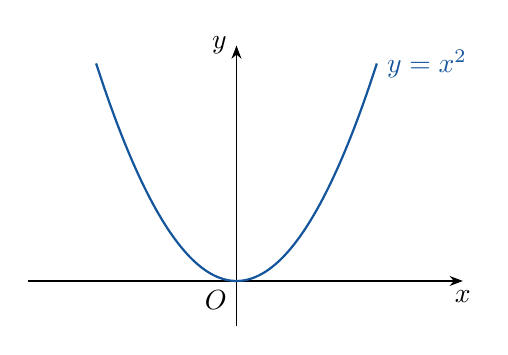
\begin{tikzpicture}[scale=1.15, >=Stealth]
    \draw[->] (-2.3,0) -- (2.5,0) node[below] {$x$};
    \draw[->] (0,-0.5) -- (0,2.6) node[left] {$y$};
    \draw[thick, mainblue, domain=-1.55:1.55, samples=100]
      plot (\x, {\x*\x}) node[right] {$y=x^{2}$};
    \node[below left] at (0,0) {$O$};
  \end{tikzpicture}
  \caption{用 TikZ 绘制的 $y=x^{2}$ 图象}
  \label{fig:tikz}
\end{figure}

\subsection{方法三：并排两张图}

\figpair{demo-parabola}{$y=x^{2}-2x-3$}{demo-parabola}{对比用同图示例}{并排插图示例}{fig:pair}

\subsection{表格}

\begin{table}[H]
  \centering
  \caption{集合与元素的关系}
  \label{tab:demo}
  \begin{tabular}{ccc}
    \toprule
    $a$ & $b$ & $a+b$ \\
    \midrule
    1 & 2 & 3 \\
    4 & 5 & 9 \\
    \bottomrule
  \end{tabular}
\end{table}

表 \ref{tab:demo} 中的三线表由 \texttt{booktabs} 宏包的 \verb|\toprule|、\verb|\midrule|、\verb|\bottomrule| 构成，比默认的表格线更适合教材排版．
 删掉即可
% ============================================================

\section{插图与表格的写法}

\subsection{方法一：插入外部图片}

把图片文件放进 \texttt{images} 目录，正文里只写文件名，不写路径。XeLaTeX 下推荐 \texttt{PDF}（矢量，最清晰）和 \texttt{PNG}（位图，可透明），\texttt{JPG} 也可用，不建议 \texttt{EPS}。

\fig[0.62]{demo-parabola}{二次函数 $y=x^{2}-2x-3$ 的图象}{fig:parabola}

由图 \ref{fig:parabola} 可见，抛物线开口向上，顶点为 $(1,-4)$，与 $x$ 轴交于 $(-1,0)$ 和 $(3,0)$．

\begin{method}[图片宽度的控制]
\texttt{\textbackslash fig} 的第一个可选参数是相对版心宽度的比例：\texttt{[0.5]} 表示占半行宽，\texttt{[1.0]} 表示占满版心．文字较多的页面建议不超过 \texttt{[0.8]}．
\end{method}

\subsection{方法二：用 TikZ 直接画（数学图形首选）}

几何图形、函数图象、韦恩图这类示意图，用 TikZ 画比截图更清晰，缩放不失真，颜色和字号也能和正文统一．

\begin{figure}[H]
  \centering
  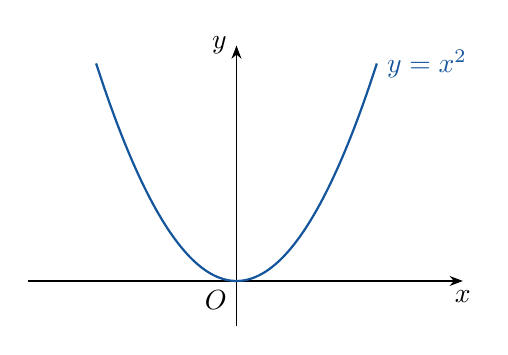
\begin{tikzpicture}[scale=1.15, >=Stealth]
    \draw[->] (-2.3,0) -- (2.5,0) node[below] {$x$};
    \draw[->] (0,-0.5) -- (0,2.6) node[left] {$y$};
    \draw[thick, mainblue, domain=-1.55:1.55, samples=100]
      plot (\x, {\x*\x}) node[right] {$y=x^{2}$};
    \node[below left] at (0,0) {$O$};
  \end{tikzpicture}
  \caption{用 TikZ 绘制的 $y=x^{2}$ 图象}
  \label{fig:tikz}
\end{figure}

\subsection{方法三：并排两张图}

\figpair{demo-parabola}{$y=x^{2}-2x-3$}{demo-parabola}{对比用同图示例}{并排插图示例}{fig:pair}

\subsection{表格}

\begin{table}[H]
  \centering
  \caption{集合与元素的关系}
  \label{tab:demo}
  \begin{tabular}{ccc}
    \toprule
    $a$ & $b$ & $a+b$ \\
    \midrule
    1 & 2 & 3 \\
    4 & 5 & 9 \\
    \bottomrule
  \end{tabular}
\end{table}

表 \ref{tab:demo} 中的三线表由 \texttt{booktabs} 宏包的 \verb|\toprule|、\verb|\midrule|、\verb|\bottomrule| 构成，比默认的表格线更适合教材排版．
 删掉即可
% ============================================================

\section{插图与表格的写法}

\subsection{方法一：插入外部图片}

把图片文件放进 \texttt{images} 目录，正文里只写文件名，不写路径。XeLaTeX 下推荐 \texttt{PDF}（矢量，最清晰）和 \texttt{PNG}（位图，可透明），\texttt{JPG} 也可用，不建议 \texttt{EPS}。

\fig[0.62]{demo-parabola}{二次函数 $y=x^{2}-2x-3$ 的图象}{fig:parabola}

由图 \ref{fig:parabola} 可见，抛物线开口向上，顶点为 $(1,-4)$，与 $x$ 轴交于 $(-1,0)$ 和 $(3,0)$．

\begin{method}[图片宽度的控制]
\texttt{\textbackslash fig} 的第一个可选参数是相对版心宽度的比例：\texttt{[0.5]} 表示占半行宽，\texttt{[1.0]} 表示占满版心．文字较多的页面建议不超过 \texttt{[0.8]}．
\end{method}

\subsection{方法二：用 TikZ 直接画（数学图形首选）}

几何图形、函数图象、韦恩图这类示意图，用 TikZ 画比截图更清晰，缩放不失真，颜色和字号也能和正文统一．

\begin{figure}[H]
  \centering
  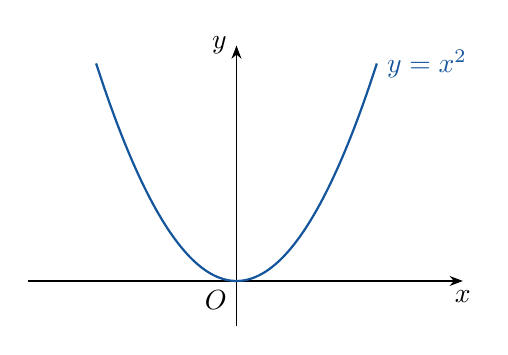
\begin{tikzpicture}[scale=1.15, >=Stealth]
    \draw[->] (-2.3,0) -- (2.5,0) node[below] {$x$};
    \draw[->] (0,-0.5) -- (0,2.6) node[left] {$y$};
    \draw[thick, mainblue, domain=-1.55:1.55, samples=100]
      plot (\x, {\x*\x}) node[right] {$y=x^{2}$};
    \node[below left] at (0,0) {$O$};
  \end{tikzpicture}
  \caption{用 TikZ 绘制的 $y=x^{2}$ 图象}
  \label{fig:tikz}
\end{figure}

\subsection{方法三：并排两张图}

\figpair{demo-parabola}{$y=x^{2}-2x-3$}{demo-parabola}{对比用同图示例}{并排插图示例}{fig:pair}

\subsection{表格}

\begin{table}[H]
  \centering
  \caption{集合与元素的关系}
  \label{tab:demo}
  \begin{tabular}{ccc}
    \toprule
    $a$ & $b$ & $a+b$ \\
    \midrule
    1 & 2 & 3 \\
    4 & 5 & 9 \\
    \bottomrule
  \end{tabular}
\end{table}

表 \ref{tab:demo} 中的三线表由 \texttt{booktabs} 宏包的 \verb|\toprule|、\verb|\midrule|、\verb|\bottomrule| 构成，比默认的表格线更适合教材排版．


% ---------------- 参考答案 ----------------
% ============================================================
%  参考答案与提示
% ============================================================

\newpage
\section*{参考答案与提示}

\noindent{\heiti 练习 1.1}\quad C

\smallskip
\noindent{\heiti 练习 1.2}\quad $B=\set{2,3,4}$．

\smallskip
\noindent{\heiti 练习 1.3}\quad 由 $3\in M$，分三种情况讨论：

（1）若 $a=3$，则 $M=\set{1,3,6}$，三个元素互不相同，符合题意；

（2）若 $a^{2}-a=3$，即 $a^{2}-a-3=0$，解得 $a=\dfrac{1\pm\sqrt{13}}{2}$．此时 $M=\set{1,\,a,\,3}$，且 $a\ne 1$、$a\ne 3$，符合题意；

（3）若 $1=3$，不成立．

综上，$a=3$ 或 $a=\dfrac{1\pm\sqrt{13}}{2}$．

\smallskip
\noindent{\heiti 练习 1.4}\quad 分两种情况：

（1）当 $a=0$ 时，方程化为 $2x+1=0$，只有一个解 $x=-\dfrac{1}{2}$，此时 $A=\set{-\dfrac{1}{2}}$，符合题意；

（2）当 $a\ne 0$ 时，方程为一元二次方程，$A$ 中只有一个元素等价于 $\Delta=4-4a=0$，解得 $a=1$，此时 $A=\set{-1}$．

综上，$a=0$ 或 $a=1$．


\end{document}
